\documentclass[Afour,sageh,times,doublespace]{sagej}

\usepackage{amsmath,amssymb}

\def\volumeyear{2026}

\begin{document}

\runninghead{Two Paths Out of Imbalance --- Online Appendix}

\title{Online Appendix: Two Paths Out of Imbalance --- How Competing Exits Produce Persistence in Interstate Relations, 1816--2012}

\author{[Author information removed for peer review]}

\begin{abstract}
This online appendix accompanies ``Two Paths Out of Imbalance: How Competing Exits Produce Persistence in Interstate Relations, 1816--2012.'' It reports full detail for the robustness and endogeneity checks summarized in the main text (Sections 3.4 and 4.5), together with additional descriptive and diagnostic material referenced there.
\end{abstract}

\maketitle

This appendix reports robustness, sensitivity, and diagnostic analyses referenced in the main text.

\section*{A1. Duration dependence in the primary hazard specification}

The primary hazard models reported in the main text (Table 2) include spell-duration fixed effects: dummy variables for the number of years since the spell began (year 1, year 2, year 3, years 4-5, years 6-10, years 11+), rather than leaving the baseline hazard unmodeled. This was added because the cumulative-incidence pattern in Figure 2 suggests transitions cluster early in a spell's life. Without an explicit duration control, a purely temporal pattern like this risks being partly absorbed by whichever time-varying network covariate happens to correlate with it, rather than reflecting that covariate's own effect.

Duration dependence is real and substantively large. A likelihood-ratio test comparing the models with and without the six-category duration fixed effects is highly significant for both hazards (dissolution: $\chi^2$=101.2, df=5, p$<$.001; realignment: $\chi^2$=737.2, df=5, p$<$.001). The duration coefficients decline broadly: a triad is markedly less likely to realign the longer it has already remained unbalanced, consistent with the ``early resolution or persistence'' pattern visible descriptively in Figure 2.

None of the paper's substantive conclusions depend on this. Every structural coefficient reported in Table 2 is estimated jointly with the duration fixed effects; the duration-adjusted and duration-naive estimates for triadic embeddedness, actor constraint, and capability are within a few percent of one another in both hazards, with no change in sign or significance level.

\begin{table*}[t]
\centering
\textbf{Table A1.} Dissolution hazard estimates without vs.\ with spell-duration fixed effects.

\vspace{4pt}
{\small\sf
\begin{tabular}{lrr}
\toprule
Predictor & Without duration control & With duration control (primary, Table 2)\\
\midrule
Triadic embeddedness & -2.455*** (0.164) & -2.508*** (0.161)\\
Tie betweenness & -0.003 (0.063) & 0.026 (0.054)\\
Actor constraint & -0.488*** (0.092) & -0.496*** (0.089)\\
Capability (log CINC) & 0.554*** (0.087) & 0.529*** (0.083)\\
\bottomrule
\end{tabular}
\par}
\end{table*}

\begin{table*}[t]
\centering
\textbf{Table A2.} Realignment hazard estimates without vs.\ with spell-duration fixed effects.

\vspace{4pt}
{\small\sf
\begin{tabular}{lrr}
\toprule
Predictor & Without duration control & With duration control (primary, Table 2)\\
\midrule
Triadic embeddedness & 0.444*** (0.058) & 0.439*** (0.046)\\
Tie betweenness & -0.023 (0.037) & -0.027 (0.031)\\
Actor constraint & 0.281*** (0.057) & 0.220*** (0.049)\\
Capability (log CINC) & -0.203*** (0.034) & -0.201*** (0.028)\\
\bottomrule
\end{tabular}
\par}
\end{table*}

The full duration-dummy coefficients are reported directly in main-text Table 2 (reference category: spell's first year at risk).

The realignment hazard's duration coefficients decline nearly monotonically, matching the intuition that realignment happens quickly or not at all. The dissolution hazard's pattern is less smooth, with a spike at year 3 alongside an overall decline. This specific spike has no confirmed explanation; the most plausible contributor is sampling noise from the much smaller number of dissolution events (678, versus 5,419 realignments) available to estimate six duration categories precisely. Every other row is consistent with the broader declining pattern. Duration here is a nuisance parameter to be modeled correctly, not a competing explanation for the embeddedness or actor-constraint effects, and it is included in every hazard specification reported in the main text and appendix from this point on (Table 2; Section 4.5's trade, contiguity, and regime-type robustness checks; and Section A11 below).

\section*{A2. Robustness to concentration in major multilateral alliance blocs}

Section A7 below documents that a handful of large multilateral alliances, coded as complete dyadic cliques among their signatories, dominate the \emph{pre-1945} closed-triad population. The same mechanism, checked against every multilateral alliance in the Gibler (2009) dataset with 8 or more members (19 instruments in total: not just the three pre-1945 instruments, but also NATO, the Warsaw Pact, the Rio Pact [Inter-American Treaty of Reciprocal Assistance, 35 members], the Arab League's joint-defense instruments, SEATO, the post-Soviet CIS/CSTO pacts, and several regional African defense pacts), has a much larger footprint across the \emph{full} 1816-2012 panel. 87.6\% of the triad-years in the primary risk table (8,913 of 10,170) fall within one of these blocs at the time, and 86.5\% of the underlying 6,277 spells (5,432) touch one of them at some point in their life.

Unlike the pre-1945 instruments in Section A7, this is not a spurious artifact of the data format producing triads out of nothing. NATO, the Warsaw Pact, and the Rio Pact were the organizing structure of Cold War international relations, and a triad of three NATO members being balanced is a substantively accurate description of the postwar security order rather than a coding quirk. The scale of the concentration still raises two questions, addressed in turn below.

\textbf{Bloc membership as a competing explanation.} Triadic embeddedness and current bloc membership are correlated (r=0.29) but far from redundant -- there is substantial variation in embeddedness \emph{within} bloc triads (SD=7.8, range 3-39) as well as outside them (SD=5.7, range 1-30). Three checks confirm the H1 mechanism is not an artifact of bloc structure:

\begin{itemize}
\item \emph{Excluding every bloc-touching spell entirely} leaves a small (1,220 triad-years, 531 dissolution and 256 realignment events) but still informative non-bloc subsample. Embeddedness remains highly significant and correctly signed in both hazards, though smaller in magnitude than the primary estimate: dissolution b=-0.70 (SE=0.20, p$<$.001; versus -2.51 in the primary specification), realignment b=+0.70 (SE=0.21, p$<$.001; versus +0.44 primary).
\item \emph{Adding current bloc membership as an additive control} to the full sample leaves embeddedness highly significant in both hazards (dissolution b=-1.46, p$<$1e-20; realignment b=+0.30, p$<$1e-10), while bloc membership is itself a large, independent predictor in the same direction as embeddedness (dissolution b=-1.81, p$<$1e-24; realignment b=+1.26, p$<$1e-33). This is consistent with bloc membership being one major source of high embeddedness rather than a separate, competing mechanism.
\item \emph{An embeddedness $\times$ bloc-membership interaction} shows the mechanism operates on both sides of that split, with the correct sign throughout, but at different magnitudes: outside blocs, embeddedness's effect is b=-0.78 on dissolution and b=+1.10 on realignment (both p$<$.001); inside blocs, the dissolution effect is substantially larger (effective b=-2.03, reflecting the exceptional institutional durability of formal defense-pact ties) while the realignment effect is if anything smaller (effective b=+0.33). This fits a meaningful share of ``realignment'' inside blocs reflecting formal accession events rather than the purely local, structurally-driven adjustment the theory describes, which shows up most cleanly outside bloc structures.
\end{itemize}

\textbf{Two-way clustering by bloc.} Two triads that are both entirely NATO members are not fully independent draws in the way clustering by triad\_id alone assumes, since they may share correlated shocks from the same underlying alliance structure. Re-estimating the primary hazard models' standard errors with two-way clustering (by triad\_id \emph{and} by each triad-year's primary bloc, using the Cameron-Gelbach-Miller multiway estimator) roughly doubles to triples the standard errors on triadic embeddedness relative to the primary one-way-clustered specification (dissolution: SE 0.16 to 0.32; realignment: SE 0.05 to 0.13); the coefficient remains highly significant in both hazards under this more conservative approach (dissolution p=9.4e-15; realignment p=.0009). One-way triad clustering, the primary specification reported in Table 2 and standard in this literature, is therefore optimistic about precision, but not by enough to change any substantive conclusion in the paper.

The paper's central claim --- that triadic embeddedness reduces the hazard of dissolution and increases the hazard of realignment --- survives every check above, in both direction and statistical significance, and is not an artifact of the international alliance system's concentration into a small number of major 20th- and 21st-century blocs. What does depend on this concentration is the \emph{magnitude} reported as the headline result in the main text (roughly a 92\% reduction in dissolution odds, a 55\% increase in realignment odds per standard deviation of embeddedness). Part of that magnitude, especially on the dissolution side, reflects the exceptional institutional lock-in of formal multilateral defense pacts specifically, and the exact percentage should not be extrapolated to interstate relationships in general.

\section*{A3. A cheap proxy for a two-mode view of alliance structure}

Section A2 treats the multilateral-clique concentration as something to check the primary results against. A more fundamental response would represent alliance structure as two-mode: states and alliance organizations as distinct node types, with a positive affiliation edge for membership, so that a 30-member organization contributes one node with 30 edges rather than 435 dyadized bilateral ties treated as independently as a real bilateral treaty. That redesign would require redefining the unit of balance itself (a closed ``triad'' would become a state-organization-state path rather than a Cartwright-Harary triad) and re-deriving every measure in the paper on the new structure. It is out of scope here, but a natural direction for follow-on work, noted in the Discussion.

A narrower, immediately answerable version of the same question does not require redefining balance at all: reweight each tie's embeddedness so that a shared membership in a large, diffuse organization counts for much less than a shared membership in a small, exclusive one, rather than letting a huge multilateral pact contribute as many full-strength ``triangles'' as an equivalent set of independent bilateral commitments would. For every dyad and year, I compute \emph{organization-weighted embeddedness}: for each alliance instrument O the two states jointly belong to that year, add 1/(size(O)-1) (a bilateral treaty, 2 members, contributes a full 1; a 30-member pact contributes roughly 0.03 per shared membership) and sum across every organization they share. This is the tie-level analogue of what a two-mode representation would treat as affiliation strength, without touching how balance or the triad panel itself is defined.

This alternative measure is \emph{negatively} correlated with the paper's primary embeddedness measure (r=-0.42): the two are capturing substantially different things, because the primary triangle-count measure is maximized precisely by membership in the largest cliques (more co-members means more triangles), while the organization-weighted measure specifically discounts large cliques. Used alone, the organization-weighted measure still points the theoretically predicted direction in both hazards (dissolution b=-0.12, p=.012; realignment b=+0.07, p=.009), though the dissolution effect is much weaker alone than the primary measure's, and the univariate dissolution model reproduces the actor-constraint sign reversal documented in Appendix A6: the organization-weighted measure alone does not fully substitute for the primary one. Entering both measures together in the same model, however, shows they are complementary rather than competing: both remain significant and correctly signed in both hazards (dissolution: primary b=-2.87, organization-weighted b=-0.40, both p$<$1e-13; realignment: primary b=+0.47, organization-weighted b=+0.12, both p$<$1e-5), and the primary measure's coefficient is if anything larger once the organization-weighted measure is controlled for.

This is suggestive rather than definitive: it is a proxy for what a full two-mode treatment would measure, not that treatment itself. But an alternative conception of tie strength, constructed specifically to avoid rewarding raw multilateral clique size, points the same direction as the primary measure and reinforces it rather than explaining it away.

\section*{A4. Endogeneity checks: lagged covariates and omitted-variable sensitivity bounds}

Main-text Section 3.4 reports two checks addressing the fact that triadic embeddedness, actor constraint, and unbalanced load are computed from the same yearly network that generates the outcomes, so the hazard models should be read as structural associations conditional on a rich set of controls, not causal estimates of a manipulated network property.

\textbf{Lagged covariates.} The primary specification already uses a predetermined-covariate design in the standard discrete-time sense (a spell's terminal-year covariates predict the transition observed going into the following year), but this does not resolve the deeper concern that even a ``predetermined'' covariate reflects the accumulated history of the surrounding network up to that point. As a further check, every triad-year in the primary risk table was re-matched to the SAME triad's structural covariates from one full year earlier (\texttt{year - 1}) in the full triad panel, rather than the row's own year. 824 of the 10,170 rows lack a value the year before (the triad was not yet a closed triad then) and are dropped, leaving 9,346 triad-years. The primary (contemporaneous) and lagged models are re-estimated on this identical 9,346-row sample, so the comparison is not confounded by the change in sample:

\begin{table*}[t]
\centering
\textbf{Table A3.} Triadic embeddedness estimates: contemporaneous vs.\ one-year-lagged covariates, identical 9,346-row sample.

\vspace{4pt}
{\small\sf
\begin{tabular}{lrr}
\toprule
& Contemporaneous (t) & Lagged (t-1)\\
\midrule
Dissolution: embeddedness & -2.148*** (SE 0.207) & -1.971*** (SE 0.181)\\
Realignment: embeddedness & 0.337*** (SE 0.061) & 0.306*** (SE 0.051)\\
\bottomrule
\end{tabular}
\par}
\end{table*}

(***p$<$.001 throughout; both p$<$1e-7.) Using embeddedness measured a full year before the year the primary specification already uses barely moves either coefficient, and the lagged estimates are, if anything, slightly more precisely estimated (smaller SEs) than the contemporaneous ones. This modest gain in precision is plausibly a composition effect rather than a substantive finding about lag length itself: dropping the 824 rows with no valid prior-year value removes exactly the least-established spells (a triad's first year as a closed triad has no prior-year value by construction), which are also the spells contributing the least-stable, highest-variance covariate readings, so the remaining 9,346-row sample is slightly better-behaved on both specifications, not only the lagged one. This does not resolve every form of network endogeneity a fully exogenous design would, but it is evidence against the estimates being driven by short-run reverse causation or simultaneity within the window the data can speak to.

\textbf{Cinelli and Hazlett (2020) sensitivity bounds.} The closed-form omitted-variable bounds in Cinelli and Hazlett (2020) are derived for OLS; applying them here required approximating the primary logistic hazard specification with a linear probability model (LPM) of the same functional form (\texttt{event \textasciitilde\ z\_tie\_btw + z\_tie\_emb + z\_actor\_load + z\_cinc + era + dur\_bin}, fit by \texttt{lm()} instead of \texttt{glm()}), a standard practical workaround rather than an exact result for the logistic model itself. Treating triadic embeddedness as the variable of interest and capability (log CINC) as the benchmark covariate for calibrating a plausible confounder's strength (\texttt{sensemakr} package):

\begin{table*}[t]
\centering
\textbf{Table A4.} Cinelli and Hazlett (2020) omitted-variable sensitivity bounds for triadic embeddedness, benchmarked against capability (log CINC).

\vspace{4pt}
{\small\sf
\begin{tabular}{lrr}
\toprule
& Dissolution & Realignment\\
\midrule
LPM coefficient (SE) & -0.0768 (0.0039) & 0.0966 (0.0084)\\
Partial $R^2$ of embeddedness with outcome & 3.68\% & 1.29\%\\
Robustness value, q=1 (bias to zero) & 17.72\% & 10.80\%\\
Robustness value, q=1, alpha=.05 (bias to non-significance) & 16.11\% & 9.05\%\\
Adjusted estimate at 1x capability's benchmark strength & -0.0475 (t=-11.24) & 0.0602 (t=6.57)\\
Adjusted 95\% CI at 1x benchmark & [-0.0558, -0.0392] & [0.0422, 0.0782]\\
\bottomrule
\end{tabular}
\par}
\end{table*}

An unobserved confounder would need to independently explain more than 17.7\% (dissolution) or 10.8\% (realignment) of the residual variance in \emph{both} embeddedness and the outcome to fully account for the observed effect, a substantial bar well above what most omitted variables achieve in observational network data. As a more concrete benchmark, a confounder exactly as strong as the paper's own strongest observed control (capability) would move the dissolution estimate only from -0.077 to -0.048 and the realignment estimate only from 0.097 to 0.060, in both cases leaving the adjusted confidence interval far from zero. Neither check substitutes for a truly exogenous research design, which is not available for this question with observational interstate network data. But both go beyond what a paragraph-length caveat alone could show, and indicate the paper's central associations are not fragile to the endogeneity concern.

\section*{A5. Fixed 5-year-window robustness check}

Before adopting the competing-risks design as primary (main text, Section 3.3), the same data were analyzed with a fixed-window logistic decomposition: every genuine onset of triadic imbalance (a triad-year where the triad was not unbalanced the year before, n=6,277) was followed forward exactly 5 years and coded as dissolved / flipped / frozen. This avoids the repeated-observation problem of counting every year a triad remains unbalanced as a fresh ``starting point'' (which would let chronically-unbalanced triads dominate the sample; see main analysis code for detail), but still requires committing to a specific window length.

Outcome distribution (n=6,277 onsets): dissolved 20.6\%, flipped 65.5\%, frozen 13.9\%.

\begin{table*}[t]
\centering
\textbf{Table A5.} Dissolved vs.\ flipped: logistic regression, fixed 5-year-window design, clustered SEs by triad.

\vspace{4pt}
{\small\sf
\begin{tabular}{lrrr}
\toprule
Predictor & $b$ & SE & p\\
\midrule
Tie/triad embeddedness & -1.48 & 0.09 & $<$.001\\
Tie load (bridging) & 0.05 & 0.05 & .33\\
Actor constraint & -0.61 & 0.09 & $<$.001\\
Capability (log CINC) & 0.59 & 0.06 & $<$.001\\
\bottomrule
\end{tabular}
\par}
\end{table*}

\begin{table*}[t]
\centering
\textbf{Table A6.} Frozen vs.\ flipped: logistic regression, fixed 5-year-window design, clustered SEs by triad.

\vspace{4pt}
{\small\sf
\begin{tabular}{lrrr}
\toprule
Predictor & $b$ & SE & p\\
\midrule
Tie/triad embeddedness & -0.37 & 0.09 & $<$.001\\
Tie load (bridging) & -0.21 & 0.11 & .06\\
Actor constraint & -0.23 & 0.10 & .02\\
Capability (log CINC) & 0.26 & 0.06 & $<$.001\\
\bottomrule
\end{tabular}
\par}
\end{table*}

Both contrasts point the same direction as the primary competing-risks models (main text Table 2 / Figure 3): embeddedness and actor constraint each reduce the probability of dissolving and of freezing, relative to flipping. The competing-risks design is preferred as primary because it removes the arbitrary 5-year window and uses every year of a spell, not only its onset, but the fixed-window result is included here as a robustness check against a more familiar research design.

\section*{A6. Actor constraint: the naive (tie-load-omitted) confound discussed in main-text Section 4.2}

The full joint model, including actor constraint, is main-text Table 2 directly (n=10,170; spell-duration fixed effects included). This section reports only the naive comparison referenced there.

\textbf{Naive comparison, actor constraint only} (tie/triad embeddedness omitted), illustrating the confound discussed in main-text Section 4.2. Fit on the same triad-year risk table as the primary hazard models (n=10,170), including the same spell-duration fixed effects as every other model in this appendix (Section A1), but omitting tie/triad embeddedness:

\begin{table*}[t]
\centering
\textbf{Table A7.} Dissolution hazard, actor constraint only (triadic embeddedness omitted).

\vspace{4pt}
{\small\sf
\begin{tabular}{lrrr}
\toprule
Predictor & $b$ & SE & p\\
\midrule
Actor constraint & +0.32 & 0.04 & $<$.001\\
Capability (log CINC) & 1.38 & 0.07 & $<$.001\\
\bottomrule
\end{tabular}
\par}
\end{table*}

Compare to the joint model (main text): actor constraint b=-0.50, p$<$.001. The sign flips entirely once tie/triad embeddedness is dropped from the model, illustrating the point made in Section 4.2: the two measures are correlated (r=-0.78) enough that a single-level specification misattributes the other level's effect.

\begin{table*}[t]
\centering
\textbf{Table A8.} Realignment hazard, actor constraint only (triadic embeddedness omitted).

\vspace{4pt}
{\small\sf
\begin{tabular}{lrrr}
\toprule
Predictor & $b$ & SE & p\\
\midrule
Actor constraint & -0.09 & 0.03 & .001\\
Capability (log CINC) & -0.36 & 0.03 & $<$.001\\
\bottomrule
\end{tabular}
\par}
\end{table*}

Here the naive estimate does not merely attenuate: it reverses sign cleanly and significantly (compare to the joint model's b=+0.22, p$<$.001), a sharper version of the same confound than appeared in an earlier specification without duration controls, where this coefficient had been attenuated to non-significance rather than flipped outright.

\section*{A7. Figure A1: descriptive time series, and the source of its pre-1945 volatility}

Figure A1 plots the share of closed triads that are unbalanced, year by year, 1816-2012, with point size scaled to that year's total triad count. It is included for completeness but not used as a main-text figure, in part because the pre-1945 portion swings dramatically from year to year --- not generic small-sample noise, but a specific mechanism that also bears on how the ``378,623 triad-years'' figure in Section 3.1 should be interpreted.

\begin{figure*}[t]
\centering
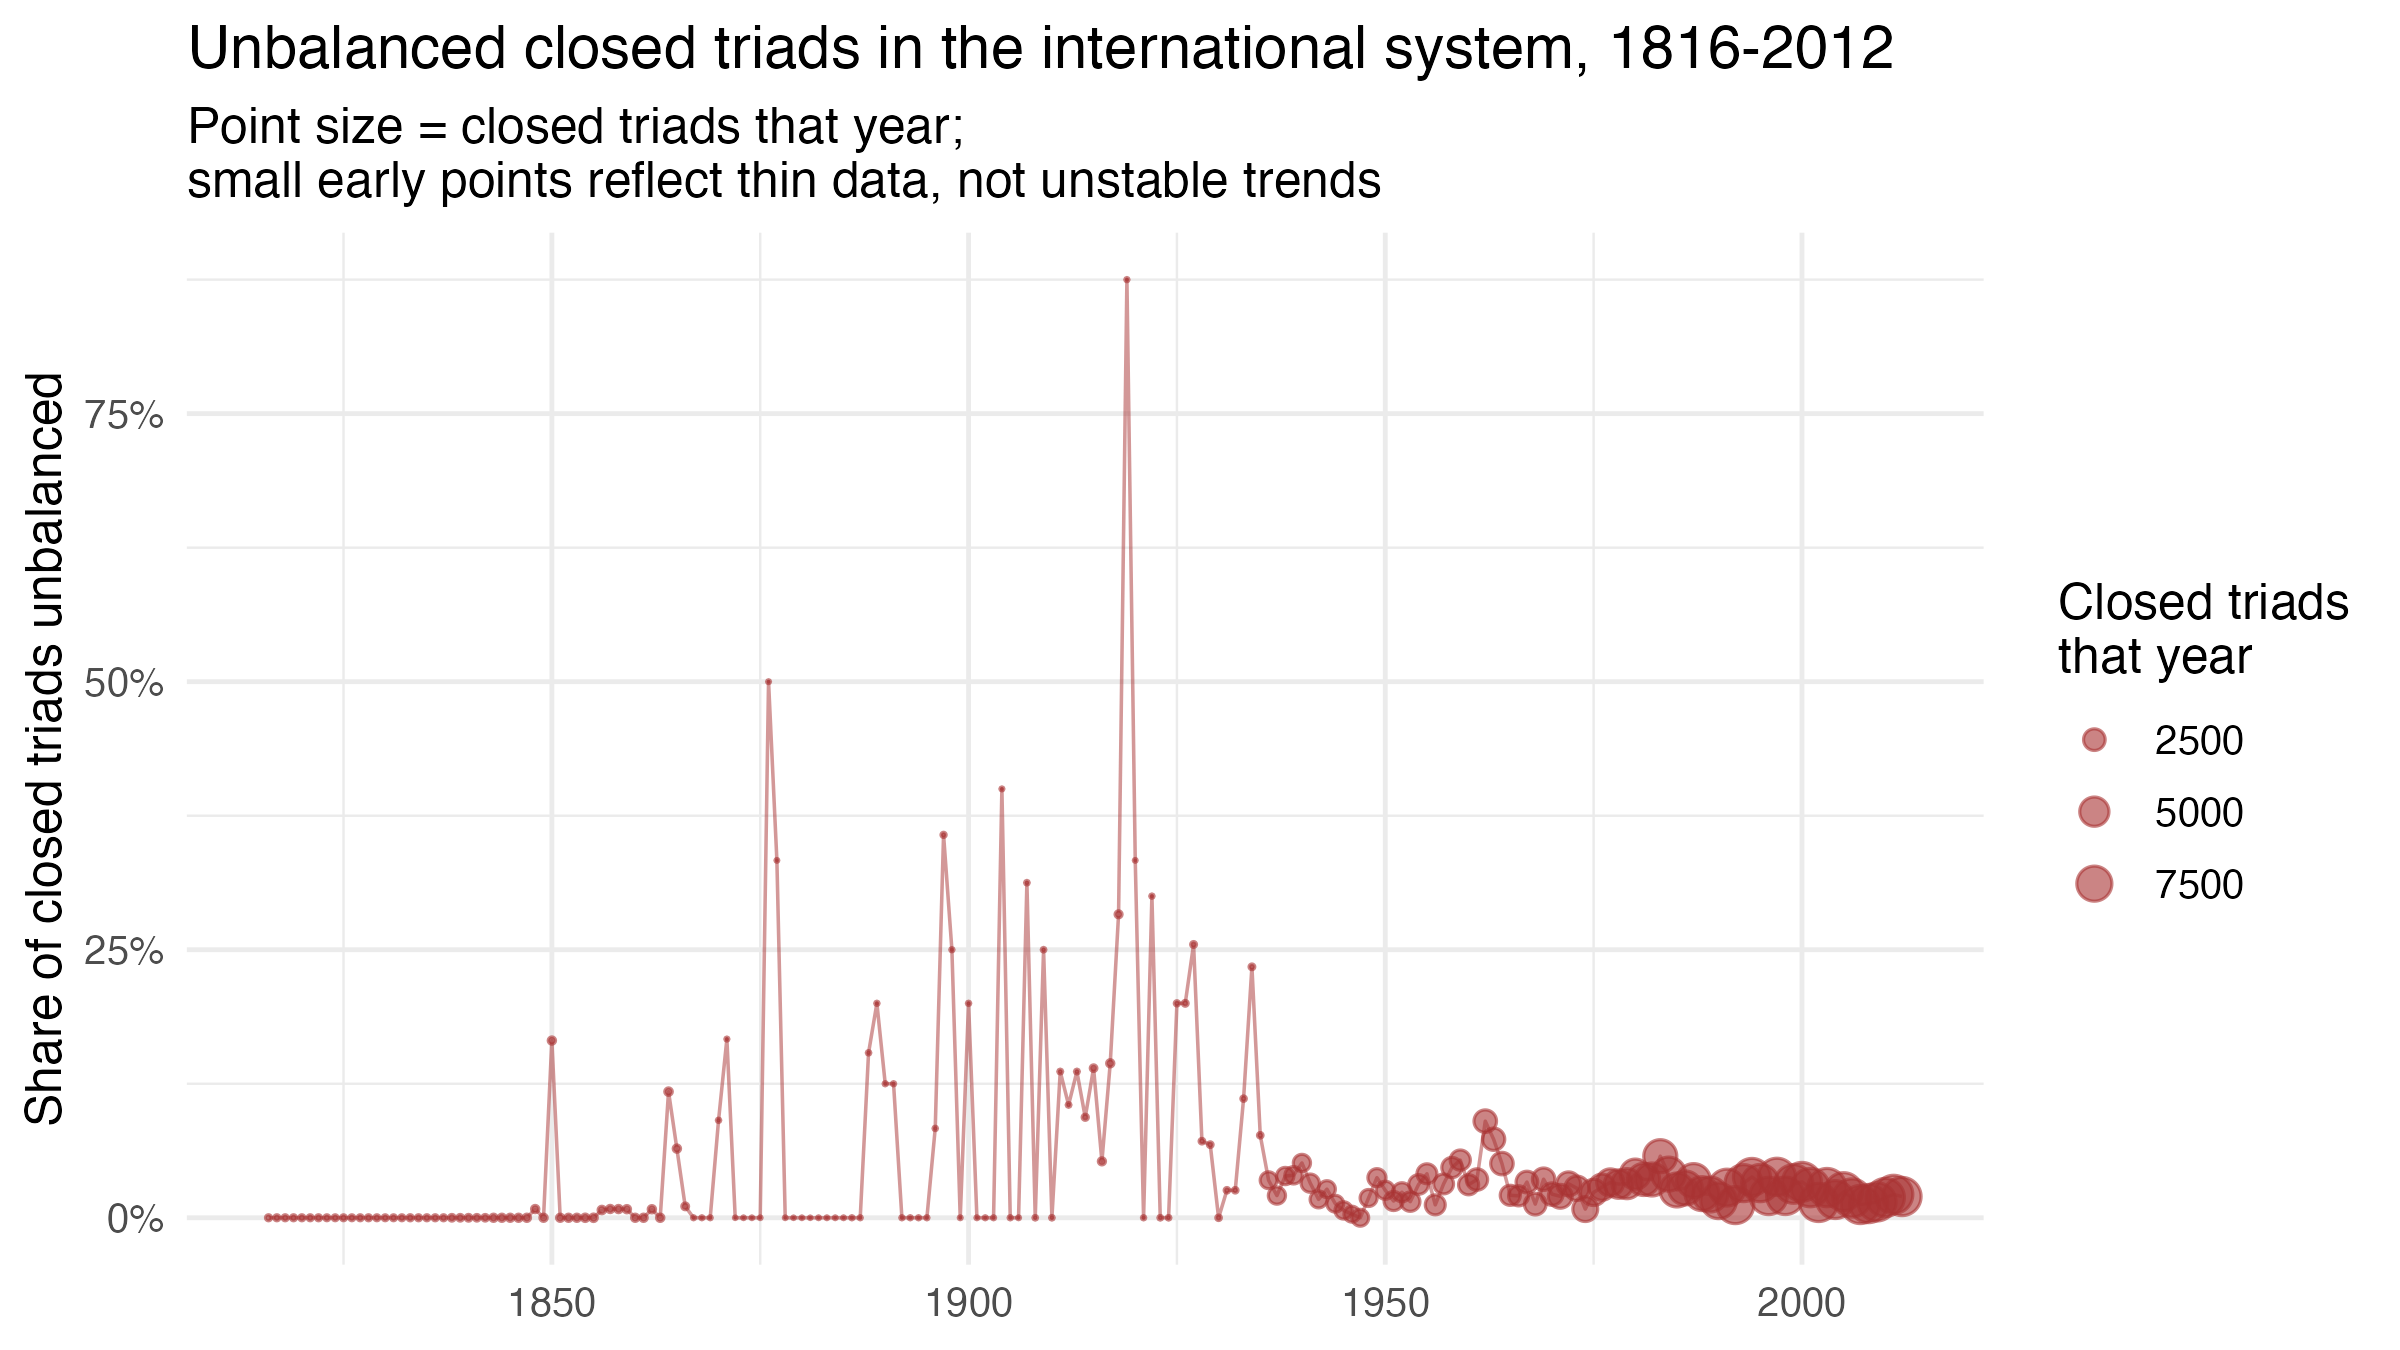
\includegraphics[width=0.75\linewidth]{../../results/fig1_imbalance_over_time.png}

\vspace{4pt}
\textbf{Figure A1.} Unbalanced closed triads in the international system, 1816--2012, descriptive time series. Point size scales with that year's total closed-triad count. Early-decade volatility reflects small annual denominators, explained by the multilateral-clique mechanism below; not load-bearing for the paper's argument, included for completeness.
\end{figure*}

\textbf{The mechanism.} The Formal Interstate Alliance dataset (Gibler 2009) codes a multilateral treaty as a complete dyadic clique: every pair of signatories receives its own bilateral alliance tie. A single N-member pact therefore contributes C(N,2) alliance dyads and, mechanically, C(N,3) closed triads the moment it enters into force, almost all of them balanced since the pact itself is entirely positive. Three such instruments dominate the pre-1945 closed-triad population: the \textbf{German Confederation} (Deutscher Bund), a 10-member Austrian- and Prussian-led mutual defense, nonaggression, and consultation pact spanning 1815-1866; the \textbf{Buenos Aires antiwar entente} of 1936, a 21-member pact linking the United States to nearly every Latin American republic; and the \textbf{Nyon Agreement} of 1937, a 9-member Mediterranean anti-piracy defense pact (Britain, France, the Soviet Union, Turkey, Greece, Yugoslavia, Romania, Bulgaria, and Egypt). Together these three instruments account for 86.6\% of all closed triad-years in the 1816-1944 portion of the panel (16,572 of 19,147). Their formation or dissolution moves the year-by-year denominator by hundreds of triads overnight, which is what actually produces Figure A1's most dramatic pre-1945 features: the near-total absence of variation from 1816 through the 1860s (the German Confederation clique alone accounts for essentially the entire closed-triad population in those decades: 120 of 121 closed triads in 1850, for instance), the collapse from 94 closed triads in 1866 to 6 in 1867 (the German Confederation dissolves in the wake of the Austro-Prussian War, which itself is visible a year earlier as a spike in negative ties among the same member states), and the jump from 39 closed triads in 1935 to 1,371 in 1936 (the Buenos Aires entente entering into force in a single year, contributing close to its full theoretical complement of C(21,3)=1,330 new closed triads). None of this is a data error: each instrument is a real historical treaty, correctly coded. But the dyadic-clique representation of a multilateral pact means these are not 120, or 1,330, independent triadic configurations coming into existence. They are one political event, multiplied combinatorially by how the data format represents it.

\textbf{A second pattern: the 1870s-1920s ``gap'' era.} The clique mechanism above explains why the denominator swings wildly; it does not by itself explain a separate pattern, that the \emph{share} unbalanced is genuinely elevated, not just noisier, for an extended stretch between the two clique eras. Averaged by decade, the share of closed triads unbalanced is near zero both before 1867 (0.1--3.0\%, the German Confederation era) and after 1936 (2.0--4.2\%, the NATO/Warsaw Pact/other 20th-century-bloc era), but runs 7.5--15.0\% throughout the 1870s--1920s, a five-decade window sitting between the two large all-positive cliques, when the diplomatic network was smaller and not yet organized into a dominant stable bloc. In absolute terms this is still a small number of triads (735 unbalanced triad-years across the entire pre-1950 period, against 9,615 from 1950 on), so this is not ``many'' unbalanced triads by any standard; it is a higher share of a much smaller population. Tracing individual years in this window to the underlying triads shows a consistent pattern: the unbalanced triads are not scattered noise but track known crises among the states that happened to have any closed triad that year. 1876 is dominated by Britain--Austria-Hungary--Russia and Britain--Russia--Ottoman Empire triads, unbalanced amid the Balkan crisis that led to the 1877--78 Russo-Turkish War; 1897 by a cluster of Britain/France/Russia/Ottoman/Greece triads during the Greco-Turkish War; 1904 by Britain--Russia--Japan, unbalanced as the Anglo-Japanese alliance of 1902 put Britain against Russia during the Russo-Japanese War; 1907 by a cluster of Central American triads coinciding with the 1906--07 Central American War; and 1919, the single highest point in the figure at 87.5\%, almost entirely by Russia's simultaneous hostility toward Britain, Germany, France, Poland, Japan, and the Baltic states during the Russian Civil War and Allied intervention. The pattern is therefore substantive as well as a small-sample artifact: the elevated share reflects real Great Power crisis periods playing out in a diplomatic network too small and too unconsolidated, in that specific window, to be diluted by a large all-positive alliance bloc the way the periods on either side of it are.

\textbf{Effect on the paper's actual results.} This does not affect the paper's results. The spell-based competing-risks analysis (Section 3.3) only ever draws on triads that become \emph{unbalanced}, and a multilateral peace pact is by construction almost entirely positive: it essentially never generates an unbalanced triad on its own, only when an external militarized dispute or additional signed tie supplies the first negative edge. Only 40.7\% of pre-1945 \emph{unbalanced} triad-years touch one of the three big cliques (258 of 634), a far smaller share than the 86.6\% of the raw denominator. At the level that matters for the paper's actual unit of analysis the effect is smaller still: of the 6,277 spells underlying every result in this paper, only 115 (1.8\%) ever involve a triad that overlaps one of the three cliques at any point in its life. Re-running the primary hazard models with these 115 spells excluded entirely (259 of 10,170 triad-years dropped) leaves the core results essentially unchanged: triadic embeddedness's coefficient moves from -2.508 to -2.435 in the dissolution hazard and from 0.439 to 0.423 in the realignment hazard, both still highly significant (p$<$.001) and within a few percent of the primary estimates in Table 2. The mechanism described above is a real feature of the pre-1945 population rather than generic ``thin data,'' and it poses no threat to the spell-based analysis this paper's conclusions rest on.

\section*{A8. H2 tie-choice analysis: unbalanced load}

Main-text Section 4.3 reports the primary (unbalanced-load) test and its result; this appendix gives the full numbers for that measure, together with two alternative measures (total embeddedness and betweenness, in Appendix A9) that perform substantially worse and do not isolate the same source of consistency pressure.

\emph{Unbalanced load} for a tie is the number of OTHER closed triads (besides the focal one) containing that tie that are themselves unbalanced that year -- distinct from total embeddedness, which counts every overlapping triangle regardless of its own balance status.

\begin{itemize}
\item 5,419 realignment events; 5,414 (99.9\%) involve exactly one tie changing sign.
\item Unbalanced-load tie structure: all three edges exactly tied in only 0.1\% of events (vs.\ 74.6\% for total embeddedness); exactly two tied in 53.4\%; all three distinct in 46.5\% (n=2,516) -- an order of magnitude more power than the embeddedness test in Appendix A9.
\item Naive test (any tie counted, including ties): changed tie has the maximum unbalanced load in 96.7\% of events (n=5,414, p$<$.001).
\item \textbf{Primary test} (all three values distinct, n=2,516): changed tie has the maximum unbalanced load in 96.6\% of events (null=33.3\%), exact binomial p$<$2.2e-16, 95\% CI [95.8\%, 97.3\%].
\item Conditional logit (unbalanced load only, 3 alternatives per event): coefficient 0.320 (SE=0.008), exp(coef)=1.38 per unit, p$<$2e-16. Concordance 0.975.
\item Conditional logit (unbalanced load + total embeddedness + betweenness): unbalanced-load coefficient 0.322 (SE=0.009), exp(coef)=1.38, p$<$2e-16 -- essentially unchanged from the univariate model. Embeddedness's own coefficient becomes small, negative, and only marginally significant once unbalanced load is included (coef=-0.064, p=.019); betweenness is not significant (coef=0.0012, p=.095). Unbalanced load, not general structural position, is doing the work.
\item Refinement (pressure proportion = unbalanced load / total embeddedness, n=2,606 with all three values distinct): changed tie has the maximum pressure proportion in 96.3\% of events (null=33.3\%), p$<$2.2e-16 -- a normalized version of the same measure gives essentially the same result.
\end{itemize}

\section*{A9. H2 tie-choice analysis: total embeddedness and betweenness as alternative measures}

The natural first measure to try, total structural embeddedness, does not distinguish balanced from unbalanced overlapping triangles, and performs far worse because it does not isolate the specific source of consistency pressure:

\begin{itemize}
\item Embeddedness, naive test (any tie): changed tie tied for the minimum in 82.9\% of events (n=5,414, p$<$.001) -- inflated almost entirely by exact ties (see below), not a meaningful ranking.
\item Embeddedness tie structure: all three edges exactly tied in 74.6\% of events (a real structural feature of dense alliance blocs sharing most of their common-neighbor count across all three edges simultaneously); exactly two tied in 22.6\%; all three distinct in only 2.7\% (n=148).
\item Embeddedness, strict test (all three distinct, n=148): changed tie is the \emph{minimum} in 27.0\% of events (null=33.3\%), p=.12 (not significant, underpowered).
\item Embeddedness, conditional logit (strict subsample): coefficient 0.023, p=.22 (not significant).
\item Betweenness tie structure: all three tied in 37\% of events (much less than embeddedness); n=1,781 events with all three betweenness values distinct.
\item Betweenness, strict test (n=1,781): changed tie has the \emph{minimum} betweenness in 24.0\% of events (null=33.3\%), p$<$.001 -- significantly BELOW chance, i.e.\ the changed tie tends to have the highest, not lowest, betweenness. Suggestive of active diplomatic management, but a much smaller and less clean effect than unbalanced load, and in the opposite direction from what either original hypothesis proposed.
\end{itemize}

\section*{A10. Dissolution disaggregation, full detail}

See main-text Section 4.3 for the summary. Full numbers:

\begin{itemize}
\item 678 dissolution events; 407 (60.0\%) involve exactly one tie disappearing, 203 (29.9\%) involve two, 68 (10.0\%) involve three.
\item Among single-tie disappearances (n=407): 326 (80.1\%) are a militarized dispute not recurring; 81 (19.9\%) are an alliance not renewed; 0 (0.0\%) coincide with either endpoint state exiting the interstate system.
\item Among multi-tie disappearances (n=271): 18 (6.6\%) coincide with at least one triad member exiting the interstate system that year.
\end{itemize}

\section*{A11. Contiguity and regime-type robustness, full models}

Restricted subsample with Polity5 coverage, n=8,076 triad-years (1850-2011), 2,118 triads. Includes the same spell-duration fixed effects as the primary specification (Section A1); full duration coefficients for this subsample omitted here for space.

\begin{table*}[t]
\centering
\textbf{Table A9.} Dissolution hazard with contiguity and regime-type controls, restricted Polity5 subsample.

\vspace{4pt}
{\small\sf
\begin{tabular}{lrrr}
\toprule
Predictor & $b$ & SE & p\\
\midrule
Triadic embeddedness & -2.60 & 0.19 & $<$.001\\
Tie betweenness & 0.15 & 0.08 & .055\\
Actor constraint & -0.36 & 0.12 & .003\\
Capability (log CINC) & 0.65 & 0.11 & $<$.001\\
Contiguity share & -0.08 & 0.07 & .25\\
Min.\ Polity2 & -0.12 & 0.08 & .154\\
\bottomrule
\end{tabular}
\par}
\end{table*}

\begin{table*}[t]
\centering
\textbf{Table A10.} Realignment hazard with contiguity and regime-type controls, restricted Polity5 subsample.

\vspace{4pt}
{\small\sf
\begin{tabular}{lrrr}
\toprule
Predictor & $b$ & SE & p\\
\midrule
Triadic embeddedness & 0.29 & 0.05 & $<$.001\\
Tie betweenness & -0.03 & 0.03 & .44\\
Actor constraint & 0.14 & 0.05 & .008\\
Capability (log CINC) & -0.26 & 0.04 & $<$.001\\
Contiguity share & -0.08 & 0.03 & .003\\
Min.\ Polity2 & 0.14 & 0.03 & $<$.001\\
\bottomrule
\end{tabular}
\par}
\end{table*}

Adding duration control leaves the core structural results intact but is not cosmetically neutral: regime type's dissolution-hazard estimate, marginal even before this check (p=.064 without duration control), is no longer distinguishable from zero once duration is properly modeled (p=.154). This is reported as it is, rather than retaining the earlier, more favorable-looking marginal estimate. Its realignment-hazard estimate remains significant either way. Contiguity's dissolution-hazard estimate was never significant and remains so; its realignment-hazard estimate is significant in both specifications.

\section*{A12. H2 under closer scrutiny: sign composition, dyad-year dependence, and an alternative load measure}

Three specific objections to the H2 unbalanced-load result (main text Section 4.3) are addressed directly here: that unbalanced load may simply be detecting which tie is the unique negative one in a two-positive-one-negative triad rather than doing independent explanatory work; that the 5,414 triad-level realignment events substantially overcount the number of independent political transitions, since one dyadic sign change can resolve many triads at once; and that unbalanced load (which counts only unbalanced overlapping triangles) omits the offsetting effect of balanced overlapping triangles, which a flip would newly unbalance. All three checks use the same single-tie-change realignment sample as Section 4.3 and Appendix A8.

\textbf{Sign composition.} Restricting to the dominant two-positive-one-negative starting configuration (5,387 of the 5,414 single-tie-change events), the negative tie is itself the maximum-unbalanced-load tie in 96.8\% of cases, and it is in fact the tie that changes in 97.3\% of cases: both numbers close to the pooled 96.6\% headline result. This follows directly from the configuration's structure: the negative tie is definitionally the one tie shared by every unbalanced triangle the triad's edges participate in, so it is structurally the most likely candidate to carry high unbalanced load regardless of any specific pressure mechanism. A conditional logit using only a negative-tie indicator (no load term at all) achieves concordance 0.977, matching unbalanced load's 0.975 and marginally exceeding it. Entering both together lifts concordance only to 0.980. Read on its own, this comparison would say unbalanced load adds essentially nothing beyond knowing which tie is currently negative.

That comparison is not decisive on its own, however, because a sign indicator is uninformative by construction whenever two of a triad's three ties share the same sign --- exactly the comparisons that would show whether unbalanced load carries information beyond sign. Restricting to same-sign tie pairs where exactly one of the pair changed (n=137 comparable pairs, ties on unbalanced load itself excluded), the higher-unbalanced-load tie of the pair is the one that changed in 75.2\% of cases (95\% CI [67.1\%, 82.2\%], exact binomial p$<$.001 against a 50\% null). Unbalanced load therefore predicts which tie changes beyond sign alone. This same-sign comparison, not the pooled 96.6\% figure, is the cleaner estimate of the construct's own contribution, since the pooled figure is inflated by a near-mechanical feature of the dominant triad configuration; the main text (Section 4.3) leads with this more conservative estimate rather than the pooled hit rate alone.

\textbf{Dyad-year dependence.} The 5,414 single-tie-change realignment events arise from only 492 unique (changed dyad, year) transitions --- a median of 10 triads resolved per transition, and as many as 46. Half of all transitions (50.6\%) resolve 10 or more triads simultaneously; only 26.8\% resolve exactly one. This is the same combinatorial phenomenon documented for the raw triad-year denominator in Appendix A7 (one multilateral treaty entering into force generates hundreds of triads from a single political event) operating on the realignment side: one dyadic sign change, inside a dense alliance bloc, can simultaneously resolve every unbalanced triad that shares that dyad. The primary strict test (all three ties' unbalanced load distinct, n=2,516) is generated by only 241 unique dyad-year transitions.

This affects how much confidence the 96.6\% figure deserves, though it does not overturn it. A cluster bootstrap resampling dyad-year transitions (not individual triad-events) with replacement, 2,000 replications, gives a 95\% interval of [95.2\%, 97.6\%] around the observed 96.6\%, close to the naive triad-level confidence interval reported in the main text. The hit rate is high and consistent within as well as between transitions, so this is not simply a few large transitions dominating the count. Collapsing entirely to one row per unique dyad-year transition (n=241) and asking whether the changed dyad had the maximum unbalanced load in \emph{any} of the triads it resolved gives 80.1\%. Testing this figure against a 33.3\% chance baseline is not appropriate: once the criterion is ``maximum in at least one of several triads,'' the null probability rises with how many triads a transition touches, and is not a flat one-third. Recomputing the chance baseline per transition as $1-(2/3)^n$ for a transition resolving $n$ triads, and averaging across the 241 transitions, gives an expected 78.5\% under a no-information null, barely below the observed 80.1\%. This collapsed diagnostic is weak evidence on its own; the same-sign comparison below, which has a well-defined 50\% null throughout, carries more of the weight. The pooled 96.6\% figure's qualitative direction holds up under this check, but the \emph{effective} sample size behind it is closer to a few hundred independent political transitions than to several thousand triad-level observations, and Table 3's reported N should be read with that in mind.

\textbf{Dependence-correcting the same-sign comparison.} The same-sign test reported in the main text (Section 4.3) --- among tie pairs sharing a sign, the higher-unbalanced-load tie is the one that changed in 75.2\% of cases, n=137 --- is the paper's more conservative evidential claim for H2, so it needs the same dependence check applied to the pooled figure above. The 137 comparable pairs correspond to only 71 unique dyad-year transitions (median 1 pair per transition, up to 12). A cluster bootstrap resampling these 71 transitions with replacement, 5,000 replications, gives a 95\% interval of [63.0\%, 84.5\%] around the observed 75.2\%, wider than the naive exact-binomial interval ([67.1\%, 82.2\%]) as expected once dependence is accounted for, but still entirely above 50\%. An equivalent check, an intercept-only logistic regression with standard errors clustered on the dyad-year transition, gives a cluster-robust 95\% CI of [62.9\%, 84.4\%], consistent with the bootstrap. The same-sign result survives proper dependence correction: a handful of dyad-year transitions each contributing several correlated pairs does not explain unbalanced load's discriminating power beyond tie sign.

\textbf{Multinomial discrete-time robustness.} The primary hazard specification (main text Table 2) fits two separate cause-specific logistic models, treating the competing event as coded 0. Because realignment accounts for 5,419 of 10,170 at-risk triad-years, I also estimated a multinomial logit on the same triad-year risk table, with three mutually exclusive outcomes (persist, the reference category; dissolve; realign) and the same covariates and duration bins as the primary specification. Triadic embeddedness retains the same sign and remains highly significant in both contrasts: dissolve b=-2.354 (SE=0.127, p$<$.001), realign b=+0.284 (SE=0.042, p$<$.001) --- smaller in magnitude than the primary specification's -2.508/+0.439 (the two designs are not estimating an identical quantity: separate cause-specific logits versus a joint multinomial model), but pointing the same direction with the same statistical confidence. The primary two-logit specification is retained as the main text's headline model for interpretability and consistency with the fixed-window comparison (Appendix A5); the two approaches agree on both the sign and the significance of the embeddedness effect.

\textbf{Net balance gain as an alternative to unbalanced load.} For a tie with total embeddedness $E$ (all overlapping triangles) and unbalanced load $U$ (the subset that are themselves unbalanced), the number of currently-balanced overlapping triangles is $B = E - U$. A flip resolves the $U$ unbalanced triangles but newly unbalances the $B$ balanced ones, so the theoretically motivated net-effect quantity is $U - B$, equivalently $2U - E$. Restricted to events with all three ties' net balance gain distinct (n=2,773), the changed tie has the maximum net balance gain in 95.8\% of cases, essentially identical to unbalanced load's 96.6\% on its own strict subsample. A head-to-head conditional logit fit statistic (AIC) very slightly favors unbalanced load alone (1855.7) over net balance gain alone (1860.0). The two measures are highly correlated in practice (a tie's balanced-triangle count is small relative to its unbalanced load in the triads driving most realignment events), so net balance gain does not outperform the simpler unbalanced-load measure empirically, even though it is arguably the more complete theoretical quantity. Both are reported here for transparency; the main text retains unbalanced load as the primary measure since it performs at least as well and is more directly interpretable.

\section*{A13. H1 and the exposure/pressure distinction: does current unbalanced load explain embeddedness's realignment effect?}

Main text Section 2.2 distinguishes total triadic embeddedness, the primary H1 predictor, conceptually from unbalanced load: embeddedness as a triad-level \emph{exposure} measure (how many surrounding configurations could eventually turn unbalanced as the network evolves), unbalanced load as \emph{instantaneous} consistency pressure, which Section 2.3 isolates for the tie-choice test (H2). Whether the interstate network actually contains enough variation to separate these two conceptually distinct quantities empirically is a different question, addressed directly here: does embeddedness's positive coefficient on the realignment hazard (Table 2) survive controlling for the triad's own current unbalanced load?

\textbf{Construction.} For every triad-year in the primary risk table (the same 10,170 triad-years underlying Table 2), I compute each of the triad's three edges' unbalanced load at year $t$ --- the number of \emph{other} closed triads sharing that edge that are themselves unbalanced that year, using the full triad population exactly as in the main text's H2 construction (Section 3.2) --- and average across the triad's three edges to obtain a triad-level current unbalanced load, on the same footing as \texttt{tie\_emb\_mean}.

\textbf{The two measures are nearly collinear at this level.} Triadic embeddedness and current unbalanced load correlate at $r=0.967$ across the 10,170 triad-years (nearly identical, $r=0.959$, restricted to the 5,419 rows that are themselves realignment events). This is not a definitional identity --- embeddedness counts all overlapping triangles, unbalanced load only the unbalanced subset --- but empirically, within this risk set, the \emph{share} of a tie's overlapping triangles that are unbalanced is remarkably stable across the embeddedness distribution: the ratio of current unbalanced load to total embeddedness has a median of 0.320 and an interquartile range of [0.313, 0.324], compared to a full range of [0, 0.923]. Because the risk set is dominated by ties embedded in a handful of major alliance blocs (Section 4.5), a tie's overlapping triangles come disproportionately from the same few blocs, and roughly a third of them are unbalanced regardless of how large the bloc is --- so embeddedness and unbalanced load rise together almost one-for-one across triads, even though they need not in principle.

\textbf{Adding unbalanced load to the realignment hazard.} Entering the triad-level current unbalanced load (standardized) into the primary realignment specification (Table 2's covariates plus duration bins) gives:

\begin{table*}[t]
\centering
\textbf{Table A11.} Realignment hazard with vs.\ without current unbalanced load added to the primary specification.

\vspace{4pt}
{\small\sf
\begin{tabular}{lrr}
\toprule
 & Baseline (Table 2) & + current unbalanced load \\
\midrule
Triadic embeddedness & 0.439*** (0.046) & -0.297* (0.133) \\
Current unbalanced load & --- & 0.749*** (0.120) \\
\bottomrule
\end{tabular}
\par}
\end{table*}

The added term is itself strongly significant, and a likelihood-ratio test confirms it improves fit ($\chi^2$=68.7, df=1, p$<$.001). Unsurprisingly, given $r=0.967$ between the two predictors, entering both produces unstable coefficients (implied VIF $\approx$15): unbalanced load is strongly positive while triadic embeddedness's own coefficient changes sign and loses most of its precision. This instability is a property of the joint model, not evidence about either variable's true effect: with two regressors this closely correlated, the model cannot allocate the shared variance between them in a way that identifies which one, if either, the association actually runs through. The same pattern holds on the dissolution hazard (embeddedness moves from b=-2.51 to b=-0.98, still correctly signed but attenuated, while unbalanced load enters at b=-1.60, p$<$.001; LRT $\chi^2$=71.2, df=1, p$<$.001).

\textbf{Reading this result.} These estimates cannot identify whether embeddedness's association with realignment operates through contemporaneous imbalance pressure or through a distinct exposure mechanism; a coefficient comparison between two regressors this collinear simply is not informative on that question. What the check does establish is that, empirically, total embeddedness and current unbalanced load are nearly redundant \emph{between} triads in this risk set --- which is exactly why the paper's actual test of the exposure/pressure distinction is designed at a different level. Section 4.3's H2 test compares the three edges \emph{within} the same triad, where total embeddedness is close to constant (74.6\% of realignment events have it exactly tied across all three edges, Section 3.2) precisely because same-bloc edges share similar overlapping-triangle counts, while unbalanced load still varies sharply across those same three edges and predicts which one changes (96.6\% hit rate against a 33.3\% baseline, or 75.2\% in the more conservative same-sign comparison; Section 4.3). The within-triad design was already the right way to separate exposure from pressure; the between-triad regression added here shows why a simple covariate-adjustment test cannot do that job at that level, and is reported for transparency rather than as a check that ``passes'' or ``fails.''

\section*{A14. Robustness to Davis's (1967) weak-balance criterion}

Main-text Section 3.1 notes that the primary analysis classifies triads as unbalanced under Cartwright and Harary's (1956) strong-balance criterion (sign product negative), which counts both the two-positive/one-negative configuration and the all-negative configuration as unbalanced. Davis's (1967) weak-balance criterion instead treats only the two-positive/one-negative configuration as unbalanced; an all-negative triad is balanced under weak balance, since three mutual enemies can each belong to a different faction rather than all belonging to one. Recent signed-network evidence shows that whether a given empirical pattern looks consistent with balance theory can depend on which of these two criteria is adopted (Gallo et al.~2024) and that all-negative triads are not always negligible substantively in interstate data specifically (Fritz et al.~2025). This appendix checks whether the paper's H1 result survives reclassifying all-negative triads as balanced.

\textbf{Reclassification.} Of the 10,350 triad-years classified unbalanced under strong balance, 10,053 (97.13\%) are the two-positive/one-negative configuration and 297 (2.87\%) are all-negative. Weak balance reclassifies exactly these 297 triad-years as balanced; every two-positive/one-negative triad-year is unbalanced under both criteria, so the two classifications agree everywhere else.

\textbf{Rebuilding the spell structure.} Because spell onset, continuation, and termination are all defined relative to whether a triad-year is unbalanced (main-text Section 3.1), reclassifying 297 triad-years changes the spell structure itself, not just a covariate: a spell that happened to pass through an all-negative year, or to terminate from one, is affected. Rebuilding spells from scratch under weak balance yields 6,035 unbalanced spells (versus 6,176 under strong balance) and a person-year risk table of 9,878 rows with an observed year-to-year transition (versus 10,170). The reduction is not evenly distributed across outcomes: dissolution events fall from 678 to 464 (a 31.6\% drop), while realignment events fall only from 5,419 to 5,396 (0.4\%). This asymmetry has a substantive reading rather than being an artifact of the reclassification: an all-negative triad-year is disproportionately likely to sit at the end of a spell that resolves by a tie simply lapsing rather than by a tie flipping sign, so removing all-negative years from the at-risk population removes a disproportionate share of dissolution-terminal observations specifically, along with the years that produced them.

\textbf{Re-estimating the primary hazard models.} The same cause-specific hazard specification reported in Table 2 (triadic embeddedness, actor constraint, edge betweenness, capability, era fixed effects, triad-clustered standard errors), re-estimated on the weak-balance spell structure, gives:

\begin{table*}[t]
\centering
\textbf{Table A12.} Primary hazard models re-estimated under Davis's (1967) weak-balance criterion vs.\ the paper's strong-balance criterion.

\vspace{4pt}
{\small\sf
\begin{tabular}{lrrrr}
\toprule
 & \multicolumn{2}{c}{Dissolution hazard} & \multicolumn{2}{c}{Realignment hazard} \\
 & Strong balance & Weak balance & Strong balance & Weak balance \\
\midrule
Triadic embeddedness & $-2.455^{***}$ & $-2.428^{***}$ & $0.444^{***}$ & $0.469^{***}$ \\
Actor constraint & $-0.488^{***}$ & $-0.692^{***}$ & $0.281^{***}$ & $0.356^{***}$ \\
Edge betweenness & $-0.003$ & $-0.043$ & $-0.023$ & $0.004$ \\
Log capability & $0.554^{***}$ & $0.543^{***}$ & $-0.204^{***}$ & $-0.169^{***}$ \\
\midrule
$N$ (person-years) & 10,170 & 9,878 & 10,170 & 9,878 \\
\bottomrule
\end{tabular}
\par}
\vspace{4pt}
\noindent{\footnotesize *** $p<.001$. All coefficients standardized.}
\end{table*}

Triadic embeddedness's effect is essentially unchanged on both hazards: it remains large, correctly signed, and highly significant, with point estimates within 0.03 (dissolution) and 0.025 (realignment) of the strong-balance values, despite dissolution events falling by nearly a third. Actor constraint and log capability likewise retain their sign and significance throughout, with actor constraint's magnitude if anything slightly larger under weak balance. Edge betweenness remains a weak, non-significant predictor under either criterion.

\textbf{Reading this result.} Redefining imbalance to exclude all-negative triads changes which specific triad-years and spells enter the risk set --- most consequentially, it removes a disproportionate share of the dissolution events used to estimate the dissolution hazard --- but it does not change the substantive conclusion. Embeddedness's opposing effects on dissolution and realignment are not an artifact of how the all-negative configuration happens to be classified; the same pattern, at essentially the same magnitude, holds whether the 297 all-negative triad-years in this panel are counted as unbalanced or not.

\end{document}
